% Install pygmentize (for minted):
% easy_install no longer exists, it was replaced by pip install.

% - Method 1:
% brew install python
% pip3 install Pygments (or with brew, easy_install was replaced by pip install)
% brew install pygments
%
% % https://tex.stackexchange.com/a/62003/69362
% which pygmentize --> take path and use below as first parameter
% sudo cp /opt/homebrew/bin/pygmentize /usr/local/bin/pygmentize

% - Method 2:
% sudo easy_install Pygments

\documentclass{beamer}
\usepackage [italian]{babel}
\usepackage [utf8]{inputenc}
\usepackage [T1]{fontenc}
 

\mode<presentation> {

% The Beamer class comes with a number of default slide themes
% which change the colors and layouts of slides. Below this is a list
% of all the themes, uncomment each in turn to see what they look like.

%\usetheme{default}
%\usetheme{AnnArbor}
%\usetheme{Antibes}
%\usetheme{Bergen}
%\usetheme{Berkeley}
%\usetheme{Berlin}
%\usetheme{Boadilla}
\usetheme{CambridgeUS}
%\usetheme{Copenhagen}
%\usetheme{Darmstadt}
%\usetheme{Dresden}
%\usetheme{Frankfurt}
%\usetheme{Goettingen}
%\usetheme{Hannover}
%\usetheme{Ilmenau}
%\usetheme{JuanLesPins}
%\usetheme{Luebeck}
%\usetheme{Madrid}
%\usetheme{Malmoe}
%\usetheme{Marburg}
%\usetheme{Montpellier}
%\usetheme{PaloAlto}
%\usetheme{Pittsburgh}
%\usetheme{Rochester}
%\usetheme{Singapore}
%\usetheme{Szeged}
%\usetheme{Warsaw}

% As well as themes, the Beamer class has a number of color themes
% for any slide theme. Uncomment each of these in turn to see how it
% changes the colors of your current slide theme.

%\usecolortheme{albatross}
%\usecolortheme{beaver}
%\usecolortheme{beetle}
%\usecolortheme{crane}
%\usecolortheme{dolphin} 
%\usecolortheme{dove}
%\usecolortheme{fly}
%\usecolortheme{lily}
%\usecolortheme{orchid}
%\usecolortheme{rose}
%\usecolortheme{seagull}
%\usecolortheme{seahorse}
%\usecolortheme{whale}
%\usecolortheme{wolverine}

%\setbeamertemplate{footline} % To remove the footer line in all slides uncomment this line
%\setbeamertemplate{footline}[page number] % To replace the footer line in all slides with a simple slide count uncomment this line
%\setbeamertemplate{navigation symbols}{} % To remove the navigation symbols from the bottom of all slides uncomment this line
}

\usepackage{listings,xcolor}
\definecolor{javared}{rgb}{0.6,0,0} % for strings
\definecolor{javagreen}{rgb}{0.25,0.5,0.35} % comments
\definecolor{javapurple}{rgb}{0.5,0,0.35} % keywords
\definecolor{javadocblue}{rgb}{0.25,0.35,0.75} % javadoc

% Colors from: "GradientDescentDiagram.png"

%\definecolor{GradientDescentDiagramBlue}{RGB}{190,208,246}
%\definecolor{GradientDescentDiagramRed}{RGB}{240,192,193}
%\definecolor{GradientDescentDiagramGreen}{RGB}{208,230,201}

% Same with saturation 40%
\definecolor{GradientDescentDiagramBlue}{RGB}{148,179,246}
\definecolor{GradientDescentDiagramGreen}{RGB}{161,230,138}
\definecolor{GradientDescentDiagramOrange}{RGB}{245,180,1}
\definecolor{GradientDescentDiagramRed}{RGB}{240,144,147}

% https://tex.stackexchange.com/questions/89821/how-to-draw-a-solid-colored-circle
\usepackage{tikz}
\newcommand{\colouredcircle}[1][black]{\tikz\draw[#1,fill=#1] (0,0) circle (.5ex);}

% https://tex.stackexchange.com/questions/147642/how-to-create-new-commands-with-multiple-arguments
% https://tex.stackexchange.com/questions/201013/how-to-include-a-background-image-to-only-one-page-of-a-beamer-presentation
\newcommand{\sectionframe}[2]{\usebackgroundtemplate{%             declare it
	\tikz[overlay,remember picture] \node[opacity=0.4, at=(current page.center)] {
	   \includegraphics[height=\paperheight,width=\paperwidth]{#1}};
	}
	\begin{frame}
		\begin{center}
			\ \newlinedouble
			\Huge \textbf{#2}
		\end{center}
	\end{frame}
	\usebackgroundtemplate{}%% undeclare it
}

\usepackage{colortbl}
\usepackage{array,multirow}
\usepackage{graphicx} % Allows including images
\usepackage{amssymb}
\usepackage{amsmath} 
\usepackage{latexsym}
\usepackage{mathtools}
\usepackage{booktabs} % Allows the use of \toprule, \midrule and \bottomrule in tables
\usepackage{amsfonts}
\usepackage{pbox}

% These two beloware for the euro symbol
% \usepackage{libertine}
\usepackage{eurosym}
\usepackage{minted}   % code prettyfier

% http://ctan.math.washington.edu/tex-archive/macros/latex/contrib/mathtools/empheq.pdf
\usepackage{empheq}

% https://en.wikibooks.org/wiki/LaTeX/Algorithms
% https://ctan.mirror.garr.it/mirrors/ctan/macros/latex/contrib/algorithm2e/doc/algorithm2e.pdf
\usepackage[]{algorithm2e}

% https://www.overleaf.com/latex/examples/drawing-coloured-boxes-using-tcolorbox/pvknncpjyfbp
\usepackage{tikz,lipsum,lmodern}
\usepackage[most]{tcolorbox} 

%\begin{tcolorbox}[colback=yellow!10,colframe=blue!40!black!60]
%  My box
%\end{tcolorbox}


% https://www.researchgate.net/publication/341380597_Insert_GIF_in_a_LaTeX_Beamer_Presentation
% options --> https://texblog.org/2018/03/05/the-animate-package/
% gif converter --> https://image.online-convert.com/convert-to-png
\usepackage{animate}

% per gestire gli if
% https://tex.stackexchange.com/a/58627/69362
% https://www.ctan.org/pkg/ifthen
\usepackage{ifthen}
\newboolean{highschool}
\setboolean{highschool}{true}
%\ifthenelse{\boolean{highschool}}{}{
%}

% Emoji
% https://tex.stackexchange.com/questions/3695/smileys-in-latex
%\usepackage{MnSymbol,wasysym}
%(\smiley ~oppure \frownie)


% Per gli svg usare la app per mac: gapplin per convertirle in png
% Su photoshop:
% C --> Cropping
% CMD + T --> una volta selezionato il layer lo puoi resizare
% per convertire svg in pdf --> usare "SVG Converter" per mac
% https://apps.apple.com/us/app/svg-converter-ohanaware-com/id1075707641?mt=12

% Init Yellow box formula
%\begin{empheq}[box=\fcolorbox{blue!40!black!60}{yellow!10}]{align*}
%\mbox{Err}_{\mathcal{TE}} = \frac{1}{n} \sum_{i=1}^m \mathbb{I}[\widetilde y_i\not= \hat C(\widetilde x_i)]
%\end{empheq}
% End Yellow box

% Init Simple formula centered (no margins)
%\makebox[\textwidth]{$\mbox{Err}_{\mathcal{TE}} = \frac{1}{n} \sum_{i=1}^m \mathbb{I}[\widetilde y_i\not= \hat C(\widetilde x_i)]$}
% End Simple Fomula centered (no margins)

% Bold in math
% $\pmb{letter}$

% Commands definitions
\newlength{\mylenxyz}\setlength{\mylenxyz}{2mm}

% Definizione di nuovi comandi

% My commands
\newcommand{\newlinedouble}{\\~\\}
\newcommand{\newlinetriple}{\\~\\~\\}
\newcommand{\mlbold}{\textbf{\ml}}
% https://tex.stackexchange.com/a/164665/69362
\newcommand\undermat[2]{% http://tex.stackexchange.com/a/102468/5764
  \makebox[0pt][l]{$\smash{\underbrace{\phantom{%
    \begin{matrix}#2\end{matrix}}}_{\text{$#1$}}}$}#2}

% https://tex.stackexchange.com/questions/249616/tex-question-about-double-underlining-in-math-mode
\def\doubleunderline#1{\underline{\underline{#1}}}


% Useful math commands

\newcommand{\rr}[1]{\textcolor{red}{\texttt{#1}}}
\newcommand{\mrr}[1]{\mbox{\textcolor{red}{\texttt{#1}}}}
\newcommand{\tg}[1]{\textcolor{green}{\textit{#1}}}

\newcommand{\bb}[1]{\textbf{#1}}
\newcommand{\ii}[1]{\textit{#1}}
\newcommand{\xt}[1]{\texttt{#1}}
\newcommand{\traccia}[1]{\ensuremath{\mbox{{\textup{traccia}}}(#1)}}
\newcommand{\rango}[1]{\ensuremath{\mbox{{\textup{rango}}}(#1)}}
\renewcommand{\vec}[1]{\ensuremath{\mbox{{\textup{vec}}}(#1)}}
\newcommand{\num}{\ensuremath{\mbox{{\textup{num}}}}}
\newcommand{\prob}{\ensuremath{\mbox{{\textup{Prob}}}}}
\newcommand{\E}{\ensuremath{\mbox{{\textup{E}}}}}
\newcommand{\Var}{\ensuremath{\mbox{{\textup{Var}}}}}
\newcommand{\se}{\ensuremath{\mbox{{\textup{SE}}}}}
\newcommand{\Cov}{\ensuremath{\mbox{{\textup{Cov}}}}}
\newcommand{\Corr}{\ensuremath{\mbox{{\textup{Corr}}}}}
\newcommand{\plim}{\ensuremath{\mbox{p}\!\lim}}
\newcommand{\longlongrightarrow}{\ensuremath{-\!\!-\!\!\!\longrightarrow}}
\newcommand{\diag}{\ensuremath{\mbox{diag}}}
\newcommand{\mbA}{\mathbf{A}}
\newcommand{\mbB}{\mathbf{B}}
\newcommand{\wmbB}{\mathbf{\widehat{B}}}
\newcommand{\smbB}{\mathbf{\scriptstyle B}}
\newcommand{\swmbB}{\mathbf{\scriptstyle \widehat{B}}}
\newcommand{\mbC}{\mathbf{C}}
\newcommand{\smbC}{\mathbf{\scriptstyle C}}
\newcommand{\mbD}{\mathbf{D}}
\newcommand{\mbE}{\mathbf{E}}
\newcommand{\mbF}{\mathbf{F}}
\newcommand{\mbI}{\mathbf{I}}
\newcommand{\mbH}{\mathbf{H}}
\newcommand{\mbM}{\mathbf{M}}
\newcommand{\mbN}{\mathbf{N}}
\newcommand{\mbP}{\mathbf{P}}
\newcommand{\mbQ}{\mathbf{Q}}
\newcommand{\mbR}{\mathbf{R}}
\newcommand{\smbR}{\mathbf{\scriptstyle R}}
\newcommand{\smbV}{\mathbf{\scriptstyle V}}
\newcommand{\mbS}{\mathbf{S}}
\newcommand{\mbT}{\mathbf{T}}
\newcommand{\mbX}{\mathbf{X}}
\newcommand{\mbW}{\mathbf{W}}
\newcommand{\smbX}{\mathbf{\scriptstyle X}}
\newcommand{\mbV}{\mathbf{V}}
\newcommand{\mbZ}{\mathbf{Z}}
\newcommand{\mbY}{\mathbf{Y}}
\newcommand{\smbZ}{\ensuremath{\mbox{\boldmath $\scriptstyle Z$}}}
\newcommand{\mbSigma}{\ensuremath{\mbox{\boldmath$\Sigma$}}}
\newcommand{\smbSigma}{\ensuremath{\mbox{\boldmath$\scriptstyle \Sigma$}}}
\newcommand{\mbLambda}{\ensuremath{\mbox{\boldmath$\Lambda$}}}
\newcommand{\mbUpsilon}{\ensuremath{\mbox{\boldmath$\Upsilon$}}}
\newcommand{\mbOmega}{\ensuremath{\mbox{\boldmath$\Omega$}}}
\newcommand{\smbOmega}{\ensuremath{\mbox{\boldmath$\scriptstyle \Omega$}}}
\newcommand{\mbPhi}{\ensuremath{\mbox{\boldmath$\Phi$}}}
\newcommand{\mbPi}{\ensuremath{\mbox{\boldmath$\Pi$}}}
\newcommand{\mbPsi}{\ensuremath{\mbox{\boldmath$\Psi$}}}
\newcommand{\mbGamma}{\ensuremath{\mbox{\boldmath$\Gamma$}}}
\newcommand{\bftheta}{\ensuremath{\mbox{\boldmath$\theta$}}}
\newcommand{\sbftheta}{\ensuremath{\mbox{\boldmath$\scriptstyle \theta$}}}
\newcommand{\bfmu}{\ensuremath{\mbox{\boldmath$\mu$}}}
\newcommand{\sbfmu}{\ensuremath{\mbox{\boldmath$\scriptstyle \mu$}}}
\newcommand{\bfiota}{\ensuremath{\mbox{\boldmath$\iota$}}}
\newcommand{\sbfiota}{\ensuremath{\mbox{\boldmath$\scriptstyle \iota$}}}
\newcommand{\bfpsi}{\ensuremath{\mbox{\boldmath$\psi$}}}
\newcommand{\sbfpsi}{\ensuremath{\mbox{\boldmath$\scriptstyle \psi$}}}
\newcommand{\bfphi}{\ensuremath{\mbox{\boldmath$\phi$}}}
\newcommand{\sbfphi}{\ensuremath{\mbox{\boldmath$\scriptstyle \phi$}}}
\newcommand{\bfkappa}{\ensuremath{\mbox{\boldmath$\kappa$}}}
\newcommand{\bfvarphi}{\ensuremath{\mbox{\boldmath$\varphi$}}}
\newcommand{\sbfvarphi}{\ensuremath{\mbox{\boldmath$\scriptstyle \varphi$}}}
\newcommand{\bfnu}{\ensuremath{\mbox{\boldmath$\nu$}}}
\newcommand{\bfpi}{\ensuremath{\mbox{\boldmath$\pi$}}}
\newcommand{\sbfpi}{\ensuremath{\mbox{\boldmath$\scriptstyle \pi$}}}
\newcommand{\bfepsilon}{\ensuremath{\mbox{\boldmath$\epsilon$}}}
\newcommand{\bfupsilon}{\ensuremath{\mbox{\boldmath$\upsilon$}}}
\newcommand{\bfvarepsilon}{\ensuremath{\mbox{\boldmath$\varepsilon$}}}
\newcommand{\bfbeta}{\ensuremath{\mbox{\boldmath$\beta$}}}
\newcommand{\sbfbeta}{\ensuremath{\mbox{\boldmath$\scriptstyle \beta$}}}
\newcommand{\bfeta}{\ensuremath{\mbox{\boldmath$\eta$}}}
\newcommand{\sbfeta}{\ensuremath{\mbox{\boldmath$\scriptstyle \eta$}}}
\newcommand{\swbfbeta}{\ensuremath{\mbox{\boldmath$\scriptstyle \widehat{\beta}$}}}
\newcommand{\wbftheta}{\ensuremath{\mbox{\boldmath$\widehat{\theta}$}}}
\newcommand{\wbfbeta}{\ensuremath{\widehat{\mbox{\boldmath$\beta$}}}}
\newcommand{\bfgamma}{\ensuremath{\mbox{\boldmath$\gamma$}}}
\newcommand{\bfdelta}{\ensuremath{\mbox{\boldmath$\delta$}}}
\newcommand{\bflambda}{\ensuremath{\mbox{\boldmath$\lambda$}}}
\newcommand{\sbflambda}{\ensuremath{\mbox{\boldmath$\scriptstyle \lambda$}}}
\newcommand{\bfzeta}{\ensuremath{\mbox{\boldmath$\zeta$}}}
\newcommand{\bfalpha}{\ensuremath{\mbox{\boldmath$\alpha$}}}
\newcommand{\sbfalpha}{\ensuremath{\mbox{\boldmath$\scriptstyle \alpha$}}}
\newcommand{\bfsigma}{\ensuremath{\mbox{\boldmath$\sigma$}}}
\newcommand{\bfomega}{\ensuremath{\mbox{\boldmath$\omega$}}}
\newcommand{\sbfomega}{\ensuremath{\mbox{\boldmath$\scriptstyle \omega$}}}
\newcommand{\wsigma}{\ensuremath{\widehat{\sigma}}}
\newcommand{\bfx}{\ensuremath{\mbox{\boldmath$x$}}}
\newcommand{\sbfx}{\ensuremath{\mbox{\boldmath$\scriptstyle x$}}}
\newcommand{\bfp}{\ensuremath{\mbox{\boldmath$p$}}}
\newcommand{\bfy}{\ensuremath{\mbox{\boldmath$y$}}}
\newcommand{\bfh}{\ensuremath{\mbox{\boldmath$h$}}}
\newcommand{\wbfy}{\ensuremath{\widehat{\mbox{\boldmath$y$}}}}
\newcommand{\bfz}{\ensuremath{\mbox{\boldmath$z$}}}
\newcommand{\sbfz}{\ensuremath{\mbox{\boldmath$\scriptstyle z$}}}
\newcommand{\bfu}{\ensuremath{\mbox{\boldmath$u$}}}
\newcommand{\wbfu}{\ensuremath{\widehat{\mbox{\boldmath$u$}}}}
\newcommand{\bfw}{\ensuremath{\mbox{\boldmath$w$}}}
\newcommand{\sbfw}{\ensuremath{\mbox{\boldmath$\scriptstyle w$}}}
\newcommand{\bfr}{\ensuremath{\mbox{\boldmath$r$}}}
\newcommand{\sbfr}{\ensuremath{\mbox{\boldmath$\scriptstyle r$}}}
\newcommand{\sbfp}{\ensuremath{\mbox{\boldmath$\scriptstyle p$}}}
\newcommand{\bfs}{\ensuremath{\mbox{\boldmath$s$}}}
\newcommand{\bfq}{\ensuremath{\mbox{\boldmath$q$}}}
\newcommand{\sbfs}{\ensuremath{\mbox{\boldmath$\scriptstyle s$}}}
\newcommand{\bfe}{\ensuremath{\mbox{\boldmath$e$}}}
\newcommand{\sbfe}{\ensuremath{\mbox{\boldmath$\scriptstyle e$}}}
\newcommand{\bff}{\ensuremath{\mbox{\boldmath$f$}}}
\newcommand{\bfg}{\ensuremath{\mbox{\boldmath$g$}}}
\newcommand{\sbff}{\ensuremath{\mbox{\boldmath$\scriptstyle f$}}}
\newcommand{\bfa}{\ensuremath{\mbox{\boldmath$a$}}}
\newcommand{\bfb}{\ensuremath{\mbox{\boldmath$b$}}}
\newcommand{\bfc}{\ensuremath{\mbox{\boldmath$c$}}}
\newcommand{\bfm}{\ensuremath{\mbox{\boldmath$m$}}}
\newcommand{\sbfm}{\ensuremath{\mbox{\boldmath$\scriptstyle m$}}}
\newcommand{\bfv}{\ensuremath{\mbox{\boldmath$v$}}}
\newcommand{\sbfv}{\ensuremath{\mbox{\boldmath$\scriptstyle v$}}}
\newcommand{\bft}{\ensuremath{\mbox{\boldmath$t$}}}
\newcommand{\sbft}{\ensuremath{\mbox{\boldmath$\scriptstyle t$}}}
\newcommand{\bfzero}{\textbf{0}}

%%%%%%%%%%%%%%%%%%%%%%%%%%%%%%%%%%%%%%%%%%%%%%%%%%%%%%%%%%%%%%%%%%%%%%%%%%%%
\newcounter{esempio}
\renewcommand{\theesempio}{\arabic{esempio}}
\newenvironment{esempio}{\refstepcounter{esempio}\begin{sloppypar}
\vspace{0.5cm}\noindent\scshape Esempio \upshape\theesempio. }{
\hspace*{\fill}$\Box$\vspace{0.6cm}\end{sloppypar}}

\newcounter{ipotesi}
\renewcommand{\theipotesi}{\arabic{ipotesi}}
\newenvironment{ipotesi}{\begin{quote} \refstepcounter{ipotesi}
\scshape Ipotesi \upshape\theipotesi. }{\hspace*{\fill}$\triangleleft$
\end{quote}}

\newcounter{proprieta}
\renewcommand{\theproprieta}{\arabic{proprieta}}
\newenvironment{proprieta}{\begin{quote}\refstepcounter{proprieta}
\scshape Propriet\`{a} \upshape\theproprieta. }{\hspace*{\fill}$\triangleleft$
\end{quote}}

\newcounter{test}
\renewcommand{\thetest}{\arabic{test}}
\newcommand{\test}{\refstepcounter{test}\ensuremath{\xi_{\thetest}}}

\newenvironment{listprop}{\begin{enumerate}
\renewcommand{\labelenumi}{\emph{(}\roman{enumi}\emph{)}}}{\end{enumerate}}

\newlength{\fntxvi} \newlength{\fntxvii}
\newcommand{\ia}[1]
{{\fontencoding{OMS}\fontfamily{cmsy}\selectfont
  \fntxvi\the\fontdimen16\font
  \fntxvii\the\fontdimen17\font
  \fontdimen16\font=2.4pt \fontdimen17\font=2.4pt
  \ensuremath{\mbox{$#1$}}
  \fontencoding{OMS}\fontfamily{cmsy}\selectfont
  \fontdimen16\font=\fntxvi \fontdimen17\font=\fntxvii}}

\newcommand{\il}[1]
{{\fontencoding{OMS}\fontfamily{cmsy}\selectfont
  \fntxvi\the\fontdimen16\font
  \fntxvii\the\fontdimen17\font
  \fontdimen16\font=3.3pt \fontdimen17\font=3.3pt
  \ensuremath{\mbox{$#1$}}
  \fontencoding{OMS}\fontfamily{cmsy}\selectfont
  \fontdimen16\font=\fntxvi \fontdimen17\font=\fntxvii}}

\newcounter{saveeqn}
\newcommand{\alphaeqn}{\setcounter{saveeqn}{\value{equation}}
\stepcounter{saveeqn}\setcounter{equation}{0}
\renewcommand{\theequation}
      {\mbox{\arabic{saveeqn}\alph{equation}}}}
\newcommand{\reseteqn}{\setcounter{equation}{\value{saveeqn}}
\renewcommand{\theequation}{\arabic{equation}}}
%%%%%%%%%%%%%%%%%%%%%%%%%%%%%%%%%%%%%%%%%%%%%%%%%%%%%%%%%%%%%%%%%%%%%%%%%%%%


\newtheorem{defn}{Definizione}
\newtheorem{thm}{Teorema}
\newtheorem{cor}[thm]{Corollario}
\newtheorem{prop}[thm]{Proposizione}
\newtheorem{oss}{Osservazione}


%Information to be included in the title page:
\title{Sistemi e Reti 3$^a$}
\author{Daniele Maddaluno}
%\institute{ShareLaTeX}
\newcommand\yearnext{\advance\year by 1 \the\year\advance\year by -1}
\newcommand\yearprev{\advance\year by -1 \the\year\advance\year by +1}
\ifthenelse{\month>8}{
\newcommand\academicyear{\the\year/\yearnext}	
}{
\newcommand\academicyear{\yearprev/\the\year}	
}
\date{\academicyear}


\begin{document}

\begin{frame}
	\titlepage % Print the title page as the first slide
\end{frame}

% Split index
% https://stackoverflow.com/questions/913966/how-to-split-table-of-contents-across-multiple-slides-with-latex-beamer
\begin{frame}[allowframebreaks]
	\frametitle{Index} % Table of contents slide, comment this block out to remove it
	\tableofcontents % Throughout your presentation, if you choose to use \section{} and \subsection{} commands, these will automatically be printed on this slide as an overview of your presentation
\end{frame}
 

%--------------------------------------------------
%	PRESENTATION SLIDES 
%--------------------------------------------------

\section[Intro]{Intro}
\sectionframe{images/covers/cover_intro.jpg}{Intro}

\subsection[Intro]{Intro}

\begin{frame}
	% \frametitle{Introduzione}	
	\begin{block}{Intro}
		\begin{itemize}
				\item Lorem ipsum dolor sit amet, consectetur adipiscing elit. Sed cursus lectus a ante consectetur vehicula eget et dui. Vivamus porttitor eget nisl vitae tristique..
				\item In varius dignissim pretium. Donec non venenatis mi. Fusce vulputate nisl sed finibus pretium:
					\begin{itemize}
						\item[--] Sed erat lectus,
						\item[--] tempor quis malesuada eu, 
						\item[--] tristique sit amet elit.
					\end{itemize}
			\end{itemize}
		Vestibulum sagittis urna vitae arcu mattis aliquam. Aliquam venenatis ex sed quam rhoncus faucibus. Pellentesque habitant morbi tristique senectus et netus et malesuada fames ac turpis egestas. Cras pharetra quis enim vel iaculis. Maecenas mattis est vulputate efficitur lacinia. Aliquam erat volutpat. Maecenas ex dolor, pretium a faucibus ut, iaculis vel nibh. Vestibulum at magna et odio dictum maximus. Maecenas vitae ipsum odio. Aliquam porttitor ante nec arcu sodales, eget vulputate est faucibus.
	\end{block}
\end{frame}
\section[I Sistemi]{I Sistemi}
\label{sec:systems}
\sectionframe{images/covers/cover_systems.jpg}{I Sistemi}

\subsection[Definizioni: sistema e stato di un sistema]{Definizioni: sistema e stato di un sistema}

\begin{frame}
	\frametitle{Definizione di sistema}
	
	\begin{block}{Sistema}
		Un \textbf{sistema} è un insieme di elementi in relazione tra di loro secondo leggi ben precise che concorrono al raggiungimento di un obiettivo comune.
	\end{block}
	\begin{block}{Stato}
		Il sistema, in base al dati ricevuti in ingresso ed alla sua natura, evolve istante dopo istante in una nuova situazione che è chiamata \textbf{stato}.
	\end{block}
\end{frame}


\begin{frame}
	\frametitle{Definizione di stato di un sistema}
	
	\begin{block}{Lo stato}
		Lo \textbf{stato} di un sistema è l'insieme di informazioni necessarie e sufficienti per descrivere le condizioni in cui si trova un sistema in un qualunque istante.\\
		\vspace{0.5em}
		Ad esempio:
		\begin{itemize}
			\item Nel sistema \textbf{automobile}:\\
				stato = velocità alla quale si trova in un dato istante (0 se è ferma).
			\item Nel sistema \textbf{aeroplano}:\\
				stato = litri di carburante nel serbatoio, il numero di giri del motore, Il livello dell’ollo ecc.
		\end{itemize}
		\vspace{0.5em}
		Leggere i valori dello stato di un sistema in un determinato momento equivale a farne una fotografia istantanea.\\
%		I valori degli ingressi, uscite e stati in un sistema, vengono memorizzati in apposite variabili che prendono il nome di variabili d'ingresso, d'uscita e di stato.
		
	\end{block}
\end{frame}


\begin{frame}
	\frametitle{Esempi di sistemi e stati}
	
	\begin{block}{Esempi di sistemi e stati}
		Potremmo paragonare lo stato di un sistema ad una fotografia del sistema in un dato istante:
		\begin{itemize}
			\item \textbf{Sistema contatore del gas}: in tale contesto lo \textbf{stato} del sistema corrisponde alla cifra dei Smc (standard metro cubo) consumati fino a quell'istante.
			\item \textbf{Sistema distributore automatico delle bibite}: in tale contesto lo \textbf{stato} del sistema corrisponde alle bibite presenti nei vari slot ed al denaro per restituire il resto presente nella macchina.
		\end{itemize}
	\end{block}
\end{frame}



\subsection[Sistemi naturali, artificiali e misti]{Sistemi naturali, artificiali e misti}
\begin{frame}
	\frametitle{Sistemi naturali, artificiali e misti}
	
	\begin{block}{È possibile catalogare i sistemi in tre grandi categorie:}
		\begin{itemize}
			\item \textbf{Sistemi naturali}: \textit{sono i sistemi esistenti in natura} .\\
			Si cita come esempio il sistema solare. Anche per il corpo umano si utilizza il termine sistema inteso come insieme di componenti che, aggregati in modo opportuno, svolgono specifiche funzioni; si hanno per esempio il sistema digerente e il sistema circolatorio.
			\item \textbf{Sistemi artificiali}: \textit{sono i sistemi creati dall'uomo}.\\
			Esempi di sistemi artificiali sono il sistema computer, un distributore di bibite, un'ascensore oppure il sistema di regolazione della temperatura dell'acqua di una piscina.
			\item \textbf{Sistemi misti}: \textit{sono sistemi naturali sui quali l’uomo è intervenuto}.\\
			Si cita come esempio il caso di un sistema destinato alla produzione di energia elettrica che viene realizzato deviando un corso d'acqua.
		\end{itemize}
	\end{block}
\end{frame}


\subsection[Inputs, states e outputs]{Inputs, states e outputs}

\begin{frame}
	\frametitle{Inputs, states e outputs}
	
	\begin{block}{Potremmo rappresentare qualunque sistema X nel seguente modo:}
		\begin{itemize}
			\item Riceve un insieme di informazioni di partenza \textbf{I} che chiameremo \textbf{inputs}.
			\item Può modificare lo/gli stato/stati \textbf{S} nel quale si può trovare in un determinato istante.
			\item Fornisce un insieme di risposte \textbf{O} che chiameremo \textbf{outputs}.
		\end{itemize}
		
		\begin{figure}[!htbp]
			\centering
			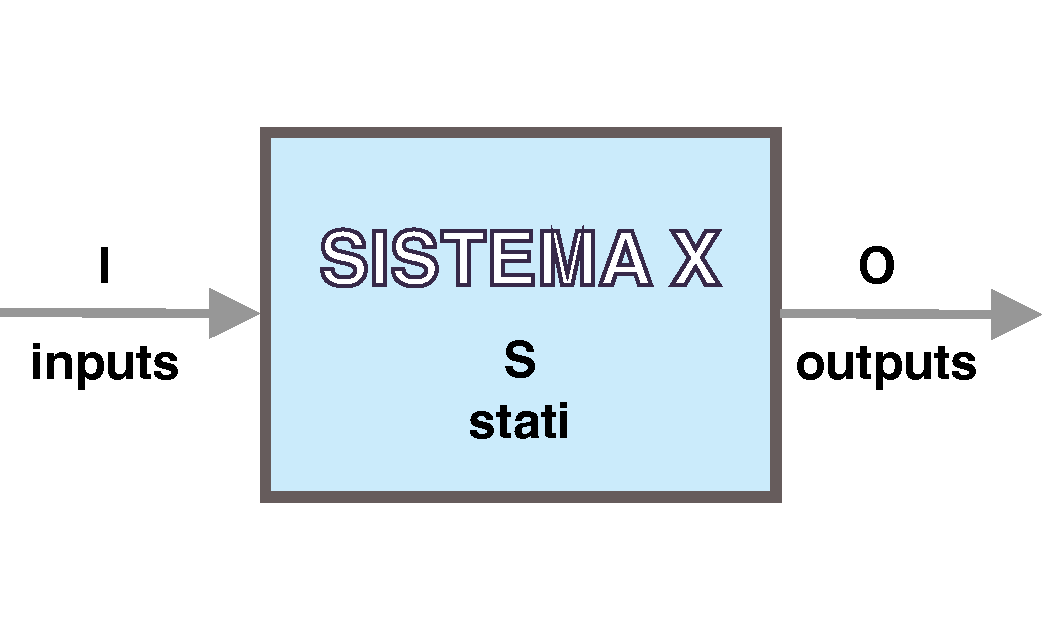
\includegraphics[width=0.55\linewidth]{images/1_i_sistemi/sistemaX.pdf}
					%\caption{}
		\end{figure}
		\vspace{0.4em}
	\end{block}
\end{frame}


\begin{frame}
	\frametitle{Inputs, states e outputs}
	
	\begin{block}{Le grandezze che determinano un sistema:}
		Un sistema è basato su quattro grandezze principali\\
		(in generale indicheremo in maiuscolo l’insieme di tutte le variabili e in minuscolo la singola variabile):\vspace{1em}
		\begin{itemize}
			\item Ingressi ($\pmb{I}$): formati dal set delle variabili di ingresso ($\pmb{i_1}$, $\pmb{i_2}$, ..., $\pmb{i_n}$)
			\item Uscite ($\pmb{O}$): formate dal set delle variabili di uscita ($\pmb{o_1}$, $\pmb{o_2}$, ..., $\pmb{o_n}$)
			\item Stati ($\pmb{S}$): formati dal set delle variabili di stato ($\pmb{s_1}$, $\pmb{s_2}$, ..., $\pmb{s_n}$)
			\item Tempo ($\pmb{T}$): formati dalle variabili tempo ($\pmb{t_1}$, $\pmb{t_2}$, ..., $\pmb{t_n}$)\\nelle quali si studia il sistema
		\end{itemize}
	\end{block}
\end{frame}


\begin{frame}
	\frametitle{Inputs, states e outputs}
	
	\begin{block}{Le grandezze che determinano un sistema:}
		\vspace{1.5em}
		\begin{figure}[!htbp]
			\centering
			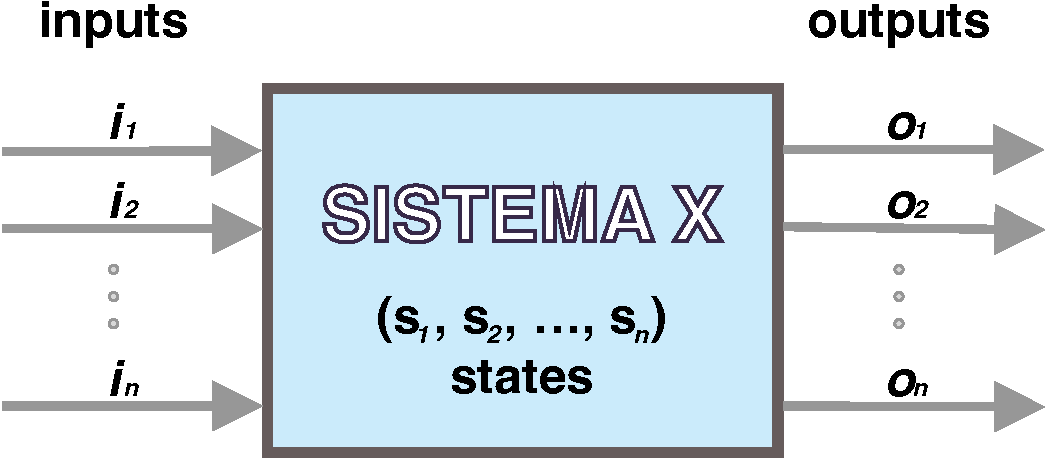
\includegraphics[width=0.65\linewidth]{images/1_i_sistemi/sistemaX2.pdf}
					%\caption{}
		\end{figure}
		\vspace{1.5em}
	\end{block}
\end{frame}



\begin{frame}
	\frametitle{Un esempio di sistema:}
	
%	\begin{block}{}
		\begin{itemize}
			\item \textbf{Set degli input}:
				\begin{itemize}
					\item[--] le monete inserite ($i_1$ = coins).
					\item[--] la scelta/selezione fatta sul distributore ($i_2$ = choice).
				\end{itemize}
			\item \textbf{Set degli stati}:
				\begin{itemize}
					\item[--] le monete all'interno del distributore ($s_1$ = coins).
					\item[--] le bibite presenti all'interno del distributore ($s_2$ = drinks).
				\end{itemize}
			\item \textbf{Set degli output}:
				\begin{itemize}
					\item[--] la bibita in uscita ($o_1$ = drink).
					\item[--] il resto ($s_2$ = change).
				\end{itemize}
		\end{itemize}
		\vspace{1.5em}
		\begin{figure}[!htbp]
			\centering
			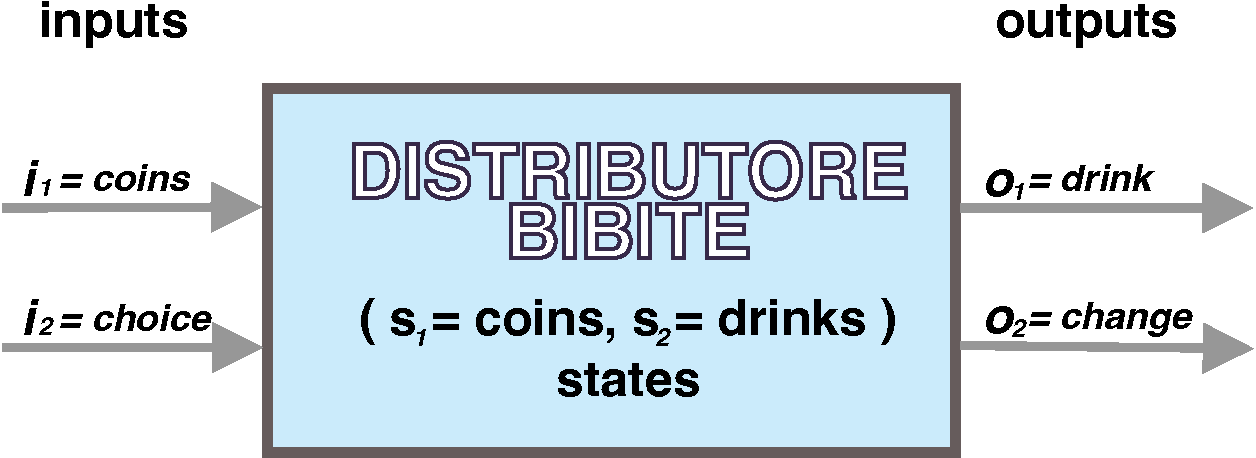
\includegraphics[width=0.60\linewidth]{images/1_i_sistemi/sistemaX3.pdf}
					%\caption{}
		\end{figure}
		\vspace{1.5em}
%	\end{block}
\end{frame}




\subsection[Funzione di transizione di stato $f$]{Funzione di transizione di stato $f$}


\begin{frame}
%	\frametitle{La funzione di transizione dello stato}
	
	\begin{block}{La \textbf{funzione di transizione dello stato} ($\pmb{f}$)}
		è la funzione che determina quale sia il valore dello stato del sistema $\pmb{s}$ in un generico istante $\pmb{t}$.
		$$\pmb{s(t) = f\Big(s(t_0), i(t)\Big)}$$
		
		\begin{itemize}
			\item $\pmb{f}$ è la funzione di transizione dello stato
			\item $\pmb{s(t_0)}$ è lo stato iniziale del sistema al tempo $t_0$
			\item $\pmb{i(t)}$ sono tutti gli ingressi applicati al sistema dall'istante iniziale $t_0$ all'istante $t$
			\item $\pmb{s(t)}$ è quindi lo stato del sistema al tempo $\pmb{t}$.	\\
			Esso può essere ottenuto tramite la funzione di transizione dello stato $\pmb{f}$ conoscendo $\pmb{s(t_0)}$ e $\pmb{i(t)}$.
		\end{itemize}
		
		\begin{figure}[!htbp]
			\centering
			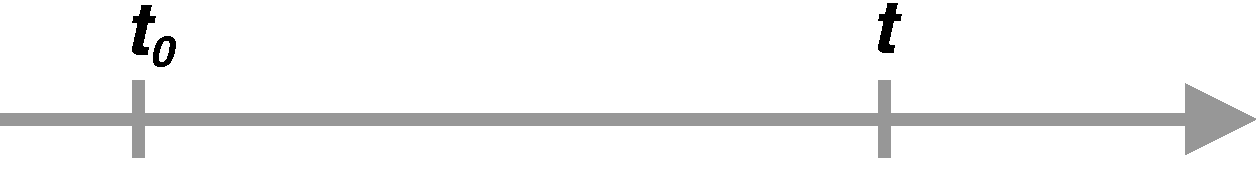
\includegraphics[width=0.50\linewidth]{images/1_i_sistemi/sistemaF.pdf}
					%\caption{}
		\end{figure}
	\end{block}
\end{frame}



\subsection[Funzione di trasformazione delle uscite $g$]{Funzione di trasformazione delle uscite}


\begin{frame}
%	\frametitle{Funzione di trasformazione delle uscite}
	
	\begin{block}{La \textbf{funzione di trasformazione delle uscite} ($\pmb{g}$)}
		è la funzione che determina quale valore avrà l'uscita $\pmb{o(t)}$ ad un generico istante $\pmb{t}$.
		$$\pmb{o(t) = g\Big(s(t), i(t)\Big)}$$
		
		\begin{itemize}
			\item $\pmb{g}$ è la funzione di trasformazione delle uscite
			\item $\pmb{s(t)}$ è lo stato del sistema al tempo $t$
			\item $\pmb{i(t)}$ sono tutti gli ingressi applicati al sistema dall'istante iniziale $t_0$ all'istante $t$
			\item $\pmb{o(t)}$ è quindi il valore che avrà l'uscita $\pmb{o(t)}$ ad un generico istante $\pmb{t}$, conoscendo il valore dello stato e degli ingressi nel medesimo istante.
		\end{itemize}
		
		\begin{figure}[!htbp]
			\centering
			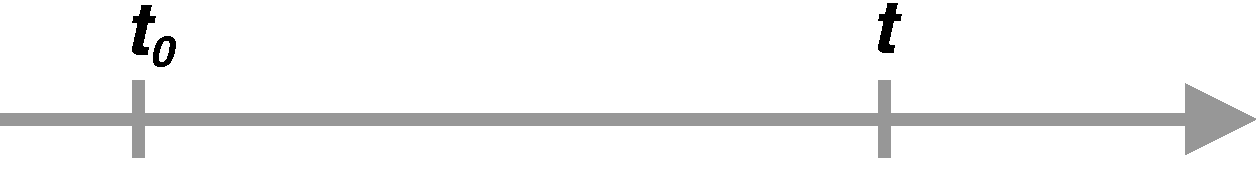
\includegraphics[width=0.50\linewidth]{images/1_i_sistemi/sistemaF.pdf}
					%\caption{}
		\end{figure}
	\end{block}
\end{frame}



\subsection[Un esempio completo]{Un esempio completo}

\begin{frame}
	\frametitle{Esempio di un sistema di illuminazione}
	\begin{block}{Sistema di illuminazione:}
	
	Prendiamo in esame un semplice sistema di illuminazione come mostrato nello schema a fianco.
	\hspace{0.3em}
	
	\begin{columns}			
		\column{0.65\linewidth}
		
		Ci sono solo quattro stati ammessi: 
		\begin{itemize}
			\item buio, ovvero tutte le luci spente ($Dark$)
			\item solo la luce nell'ingresso accesa ($L_I$)
			\item solo la luce nel corridoio a sx accesa ($L_{LX}$)
			\item solo la luce nel corridoio a dx accesa ($L_{RX}$)
		\end{itemize}
		
		Il sistema riceve gli input esclusivamente attraverso i due bottoni $B_1$ e $B_2$, possono esser premuti solo uno per volta.
		Se non mantenuti premuti rimangono sollevati (entrambi su OFF).
					
		\column{0.35\linewidth}
		\begin{figure}[!htbp]
			\centering 
			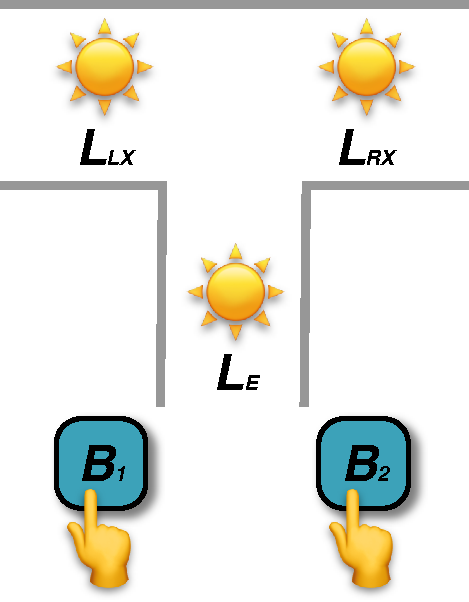
\includegraphics[width=0.8\linewidth]{images/1_i_sistemi/sistemaLight.pdf}
					%\caption{}
		\end{figure}
		
	\end{columns}
	\end{block}
\end{frame}


\begin{frame}
	\frametitle{Esempio di un sistema di illuminazione}
	\begin{block}{Sistema di illuminazione, funzione di transizione dello stato:}
	
	Prendiamo in esame la funzione di transizione dello stato del semplice sistema di illuminazione.
	
	
	\begin{columns}			
		\column{0.6\linewidth}
\begin{small}
	
\begin{table}[]
\begin{tabular}{|
>{\columncolor[HTML]{C0C0C0}}c |c|c|c|c|}
\hline
\cellcolor[HTML]{FFFFFF}$\pmb{s}$\textbackslash $\pmb{i}$ & \cellcolor[HTML]{C0C0C0}\begin{tabular}[c]{@{}c@{}}$B_1$ OFF\\ $B_2$ OFF\end{tabular} & \cellcolor[HTML]{C0C0C0}\begin{tabular}[c]{@{}c@{}}$B_1$ ON\\ $B_2$ OFF\end{tabular} & \cellcolor[HTML]{C0C0C0}\begin{tabular}[c]{@{}c@{}}$B_1$ OFF\\ $B_2$ ON\end{tabular} & \cellcolor[HTML]{C0C0C0}\begin{tabular}[c]{@{}c@{}}$B_1$ ON\\ $B_2$ ON\end{tabular} \\ \hline
$Dark$ & $Dark$ & $L_I$ & $L_I$ & - \\ \hline
$L_I$ & $L_I$ & $L_{LX}$ & $L_{RX}$ & - \\ \hline
$L_{LX}$ & $L_{LX}$ & $Dark$ & $Dark$ & - \\ \hline
$L_{RX}$ & $L_{RX}$ & $Dark$ & $Dark$ & - \\ \hline                                                                        
\end{tabular}
\end{table}
\end{small}
					
		\column{0.4\linewidth}
		\begin{figure}[!htbp]
			\centering
			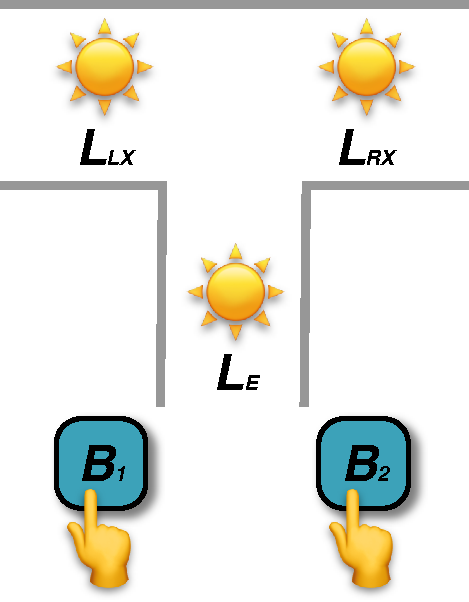
\includegraphics[width=0.80\linewidth]{images/1_i_sistemi/sistemaLight.pdf}
					%\caption{}
		\end{figure}
	\end{columns}
	\end{block}
\end{frame}




\begin{frame}
	\frametitle{Esempio di un sistema di illuminazione}
	\begin{block}{Sistema di illuminazione, funzione di transizione dello stato:}
	
	Prendiamo in esame la funzione di transizione dello stato del semplice sistema di illuminazione.
	
	
	\begin{columns}			
		\column{0.6\linewidth}
\begin{small}
	
\begin{table}[]
\begin{tabular}{|
>{\columncolor[HTML]{C0C0C0}}c |c|c|c|c|}
\hline
\cellcolor[HTML]{FFFFFF}$\pmb{s}$\textbackslash $\pmb{i}$ & \cellcolor[HTML]{C0C0C0}\begin{tabular}[c]{@{}c@{}}$B_1$ OFF\\ $B_2$ OFF\end{tabular} & \cellcolor[HTML]{C0C0C0}\begin{tabular}[c]{@{}c@{}}$B_1$ ON\\ $B_2$ OFF\end{tabular} & \cellcolor[HTML]{C0C0C0}\begin{tabular}[c]{@{}c@{}}$B_1$ OFF\\ $B_2$ ON\end{tabular} & \cellcolor[HTML]{C0C0C0}\begin{tabular}[c]{@{}c@{}}$B_1$ ON\\ $B_2$ ON\end{tabular} \\ \hline
$Dark$ & $Dark$ & $L_I$ & $L_I$ & - \\ \hline
$L_I$ & $L_I$ & $L_{LX}$ & $L_{RX}$ & - \\ \hline
$L_{LX}$ & $L_{LX}$ & $Dark$ & $Dark$ & - \\ \hline
$L_{RX}$ & $L_{RX}$ & $Dark$ & $Dark$ & - \\ \hline                                                                        
\end{tabular}
\end{table}
\end{small}
					
		\column{0.4\linewidth}
		\begin{figure}[!htbp]
			\centering
			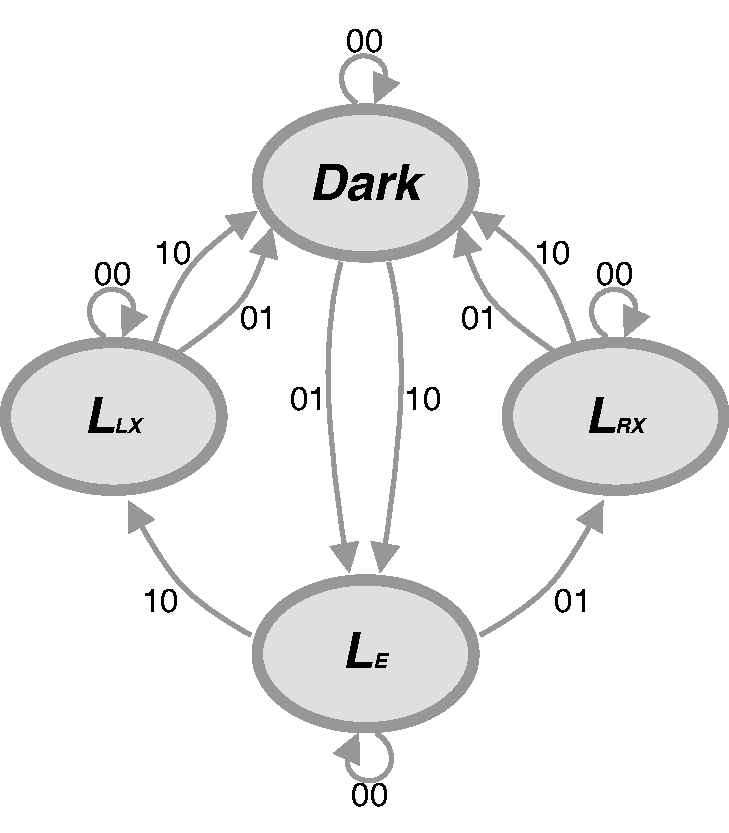
\includegraphics[width=0.9\linewidth]{images/1_i_sistemi/sistemaLightF.pdf}
					%\caption{}
		\end{figure}
	\end{columns}
	\end{block}
\end{frame}



\begin{frame}
	\frametitle{Esempio di un sistema di illuminazione}
	\begin{block}{Sistema di illuminazione, funzione di trasformazione delle uscite:}
	
	La funzione di trasformazione delle uscite in questo specifico caso è funzione solo dello stato in cui il sistema si va a trovare, ovvero non tiene di conto dell'ultimo input ricevuto al tempo $t$ ma solo dello stato:
	
	\begin{itemize}
		\item $s=Dark \quad\rightarrow$ $output =$ luci spente
		\item $s=L_{I} \quad\:\quad\rightarrow$ $output =$ luce dell'ingresso accesa
		\item $s=L_{LX} \quad\;\;\rightarrow$ $output =$ luce del corridoio sx accesa
		\item $s=L_{RX} \quad\;\;\rightarrow$ $output =$ luce del corridoio sx accesa
	\end{itemize}
	
	\end{block}
\end{frame}


 
\subsection[Classificazione dei sistemi]{Classificazione dei sistemi}

\begin{frame}
	\frametitle{Classificazione dei sistemi}
	\begin{block}{Classificazione dei sistemi:}
		L'approccio più semplice per studiare e classificare i sistemi è chiamato \textbf{modello black box} (a scatola nera).\\
		In questo modello ci si limita ad analizzare il comportamento osservabile all'esterno di un sistema ignorandone la struttura ed il funzionamento interno.
		\begin{figure}[!htbp]
			\centering
			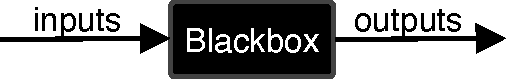
\includegraphics[width=0.8\linewidth]{images/1_i_sistemi/blackbox.pdf}
					%\caption{}
		\end{figure}
		Si esaminano quindi solo:
		\begin{itemize}
			\item gli elementi in ingresso del sistema (inputs) 
			\item gli elementi in uscita del sistema (outputs)
		\end{itemize}
%		dal sistema stesso.
	\end{block}
\end{frame}



\begin{frame}
	\frametitle{Classificazione sistemica}
	\begin{block}{Classificazione sistemica}
		Sulla base di tali osservazioni possiamo classificare un sistema identificando tipologie a due a due di natura opposta; si hanno pertanto sistemi:
		\begin{itemize}
			\item Variante o invariante
			\item Deterministico o stocastico
			\item Continuo o discreto
			\item Combinatorio o sequenziale			
			\item Proprio o improprio
			\item ...
		\end{itemize}
		
		Lo stesso sistema può anche essere classificato in modi diversi, a seconda delle caratteristiche e dell'intervallo di tempo nel quale viene studiato.\\
%		Ad es. un sistema orologio analogico (con lancette) anche se analogico, può divenire discreto quando studiato in un tempo infinitesimale ($\approx 0$)
	\end{block}
\end{frame}


\subsubsection[Variante o invariante]{Variante o invariante}
\begin{frame}
	\frametitle{Variante o invariante}
	\begin{block}{Variante o invariante nel tempo}
		Un sistema è \textbf{invariante nel tempo} quando i parametri che lo caratterizzano rimangono invarianti nel tempo e quindi le leggi che legano le sollecitazioni alle risposte rimangono invariate nel tempo.\\~\\
		\textbf{ATTENZIONE}: non è variante un sistema quando variano gli ingressi e/o le uscite: in tal caso si dice che il sistema è dinamico.
	\end{block}
\end{frame}


\subsubsection[Deterministico o stocastico]{Deterministico o stocastico}
\begin{frame}
	\frametitle{Deterministico o stocastico}
	\begin{block}{Un sistema è deterministico}
		Un sistema è \textbf{deterministico} quando le funzioni di transizione e di trasformazione permettono la determinazione del valore dello stato e delle uscite in modo univoco.
	\end{block}
	
	\begin{block}{Un sistema è stocastico}
		Un sistema è \textbf{stocastico} quando almeno una delle due funzioni è regolata da legami di natura probabilistica.
	\end{block}
\end{frame}


\subsubsection[Continuo o discreto]{Continuo o discreto}
\begin{frame}
	\frametitle{Continuo o discreto}
	\begin{block}{Continuo o discreto}
		Un sistema può essere \textbf{discreto}:
		\begin{itemize}
			\item nell'\textbf{avanzamento}
			\item nelle \textbf{sollecitazioni}
			\item nelle \textbf{interazioni}
		\end{itemize}
		
		Un sistema si dice continuo se non è discreto in nessuno dei tre aspetti (avanzamento, sollecitazioni e interazioni).
	\end{block}
\end{frame}


\begin{frame}
	\frametitle{Continuo o discreto}
	\begin{block}{Un sistema è discreto nell'avanzamento}
		quando non esistono tempi intermedi tra un istante $t_n$ e il suo successivo $t_{n+1}$ in cui viene studiato (ad es. nei sistemi di scansione temporale tramite un clock).\\
		Ad esempio: \textit{ripresa cinematografica} o \textit{microprocessore scandito dal clock}.
	\end{block}
	
	\begin{block}{Un sistema è discreto nelle sollecitazioni}
		quando l'insieme delle Variabili d'Ingresso (VI) è discreto.\\
		Ad esempio: \textit{un distributore di bibite} o \textit{un sistema di illuminazione}.
	\end{block}
	
	\begin{block}{Un sistema è discreto nelle interazioni}
		quando la funzione di transizione e/o la funzione di trasformazione sono entrambe discrete.\\
		Ad esempio: \textit{un orologio digitale con ingresso continuo ma uscita discreta}.
	\end{block}
\end{frame}


\begin{frame}
	\frametitle{Continuo o discreto}
	\begin{block}{Esempi di sistemi continui}		
		\begin{itemize}
			\item un albero che produce frutti, 
			\item una mucca che produce latte,
			\item ecc...
		\end{itemize}
		
	\end{block}
	
	\begin{block}{Esempi di sistemi discreti:}		
		\begin{itemize}
			\item un distributore di lattine, 
			\item il sistema orologio digitale, 
			\item ecc...
		\end{itemize}
	\end{block}
	
\end{frame}


\begin{frame}
	\frametitle{Continuo o discreto}
	
	\begin{block}{Esempi di sistemi discreto e continuo}		
		Un classico orologio a lancette invece, a seconda dei tempi nella quale viene studiato il sistema, può essere considerato:
		\begin{itemize}
			\item \textbf{continuo}, ipotizzando che la lancetta passi con continuità dalla posizione relativa a un secondo a quella relativa all'altro secondo (codominio della funzione di trasformazione: intervallo continuo $[0, 59.999...]$).
			\item \textbf{discreto}, ipotizzando che la lancetta avanzi di uno scatto ogni secondo (codominio della funzione di trasformazione: intervallo discreto: $[0, 1, 2, 3, 4, 5, ..., 59]$).
		\end{itemize}
	\end{block}	
\end{frame}



\subsubsection[Combinatorio o sequenziale]{Combinatorio o sequenziale}
\begin{frame}
	\frametitle{Combinatorio o sequenziale}
	\begin{block}{Un sistema è \textbf{combinatorio}}
		se le uscite dipendono solo dai valori presenti agli ingressi nel medesimo istante, le uscite non ricordano il passato: il sistema è senza memoria e le uscite sono una combinazione degli ingressi nello stesso istante
	\end{block}
	
	\begin{block}{Un sistema è \textbf{sequenziale}}
		quando le uscite dipendono non solo dai valori degli ingressi in quell'istante, ma anche dai valori assunti in precedenza dagli ingressi.
	\end{block}
	
	
\end{frame}


\begin{frame}
	\frametitle{Combinatorio o sequenziale}
	

	\begin{columns}			
		\column{0.7\linewidth}
		
		\begin{block}{Esempi di sistemi combinatori}
			\begin{itemize}
				\item \textbf{Lucchetto a combinazione numerica}:\\per ottenere la combinazione si devono ruotare e posizionare manopole rotanti ciascuna su di una cifra; è indipendente dal valore iniziale delle manopole in quanto conta solamente il numero finale sul quale vengono posizionate.
				\item \textbf{Porte logiche (and, or, not, ...)}:\\l'uscita di questi sistemi dipende unicamente dal valore presente sugli ingressi e non dai valori degli ingressi delle operazioni precedenti.
			\end{itemize}
		\end{block}
					
		\column{0.3\linewidth}
		\begin{figure}[!htbp] 
			\centering
			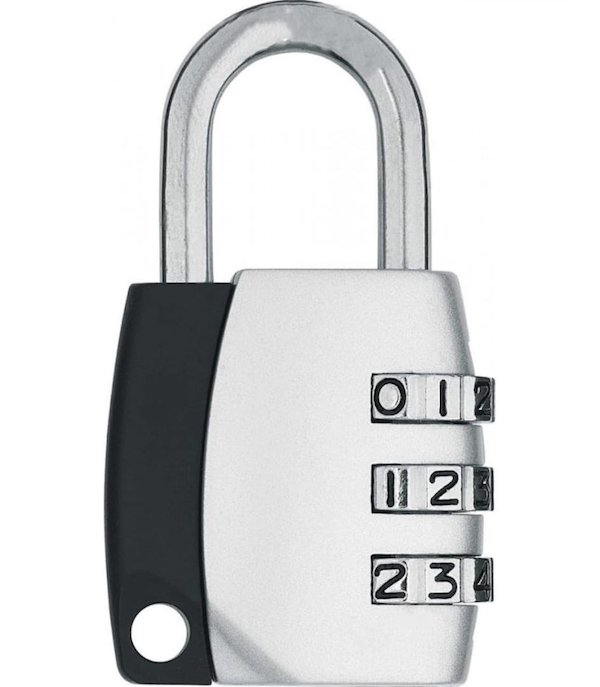
\includegraphics[width=0.7\linewidth]{images/1_i_sistemi/lock.png}
					%\caption{}
		\end{figure}
		
		\begin{figure}[!htbp]
			\centering
			\advance\rightskip-0.25cm
			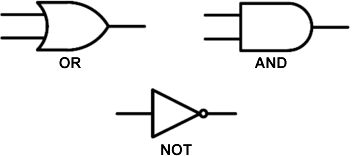
\includegraphics[width=1.0\linewidth]{images/1_i_sistemi/ports.png}
					%\caption{}
		\end{figure}
	\end{columns}
		
		
	
	
	
\end{frame}



\begin{frame}
	\frametitle{Combinatorio o sequenziale}
		
	\begin{columns}			
		\column{0.6\linewidth}
		
		\begin{block}{Esempi di sistemi sequenziali}
		\begin{itemize}
			\item \textbf{Distributore automatico di merendine}:\\sistema sequenziale in quanto erogazione del prodotto dipende dalle monete inserite precedentemente che concorrono a formare l'importo necessario (mantiene la memoria del denaro inserito)
		\end{itemize}
		\end{block}
					
		\column{0.4\linewidth}
		\begin{figure}[!htbp] 
			\centering
%			\advance\leftskip-0.25cm
			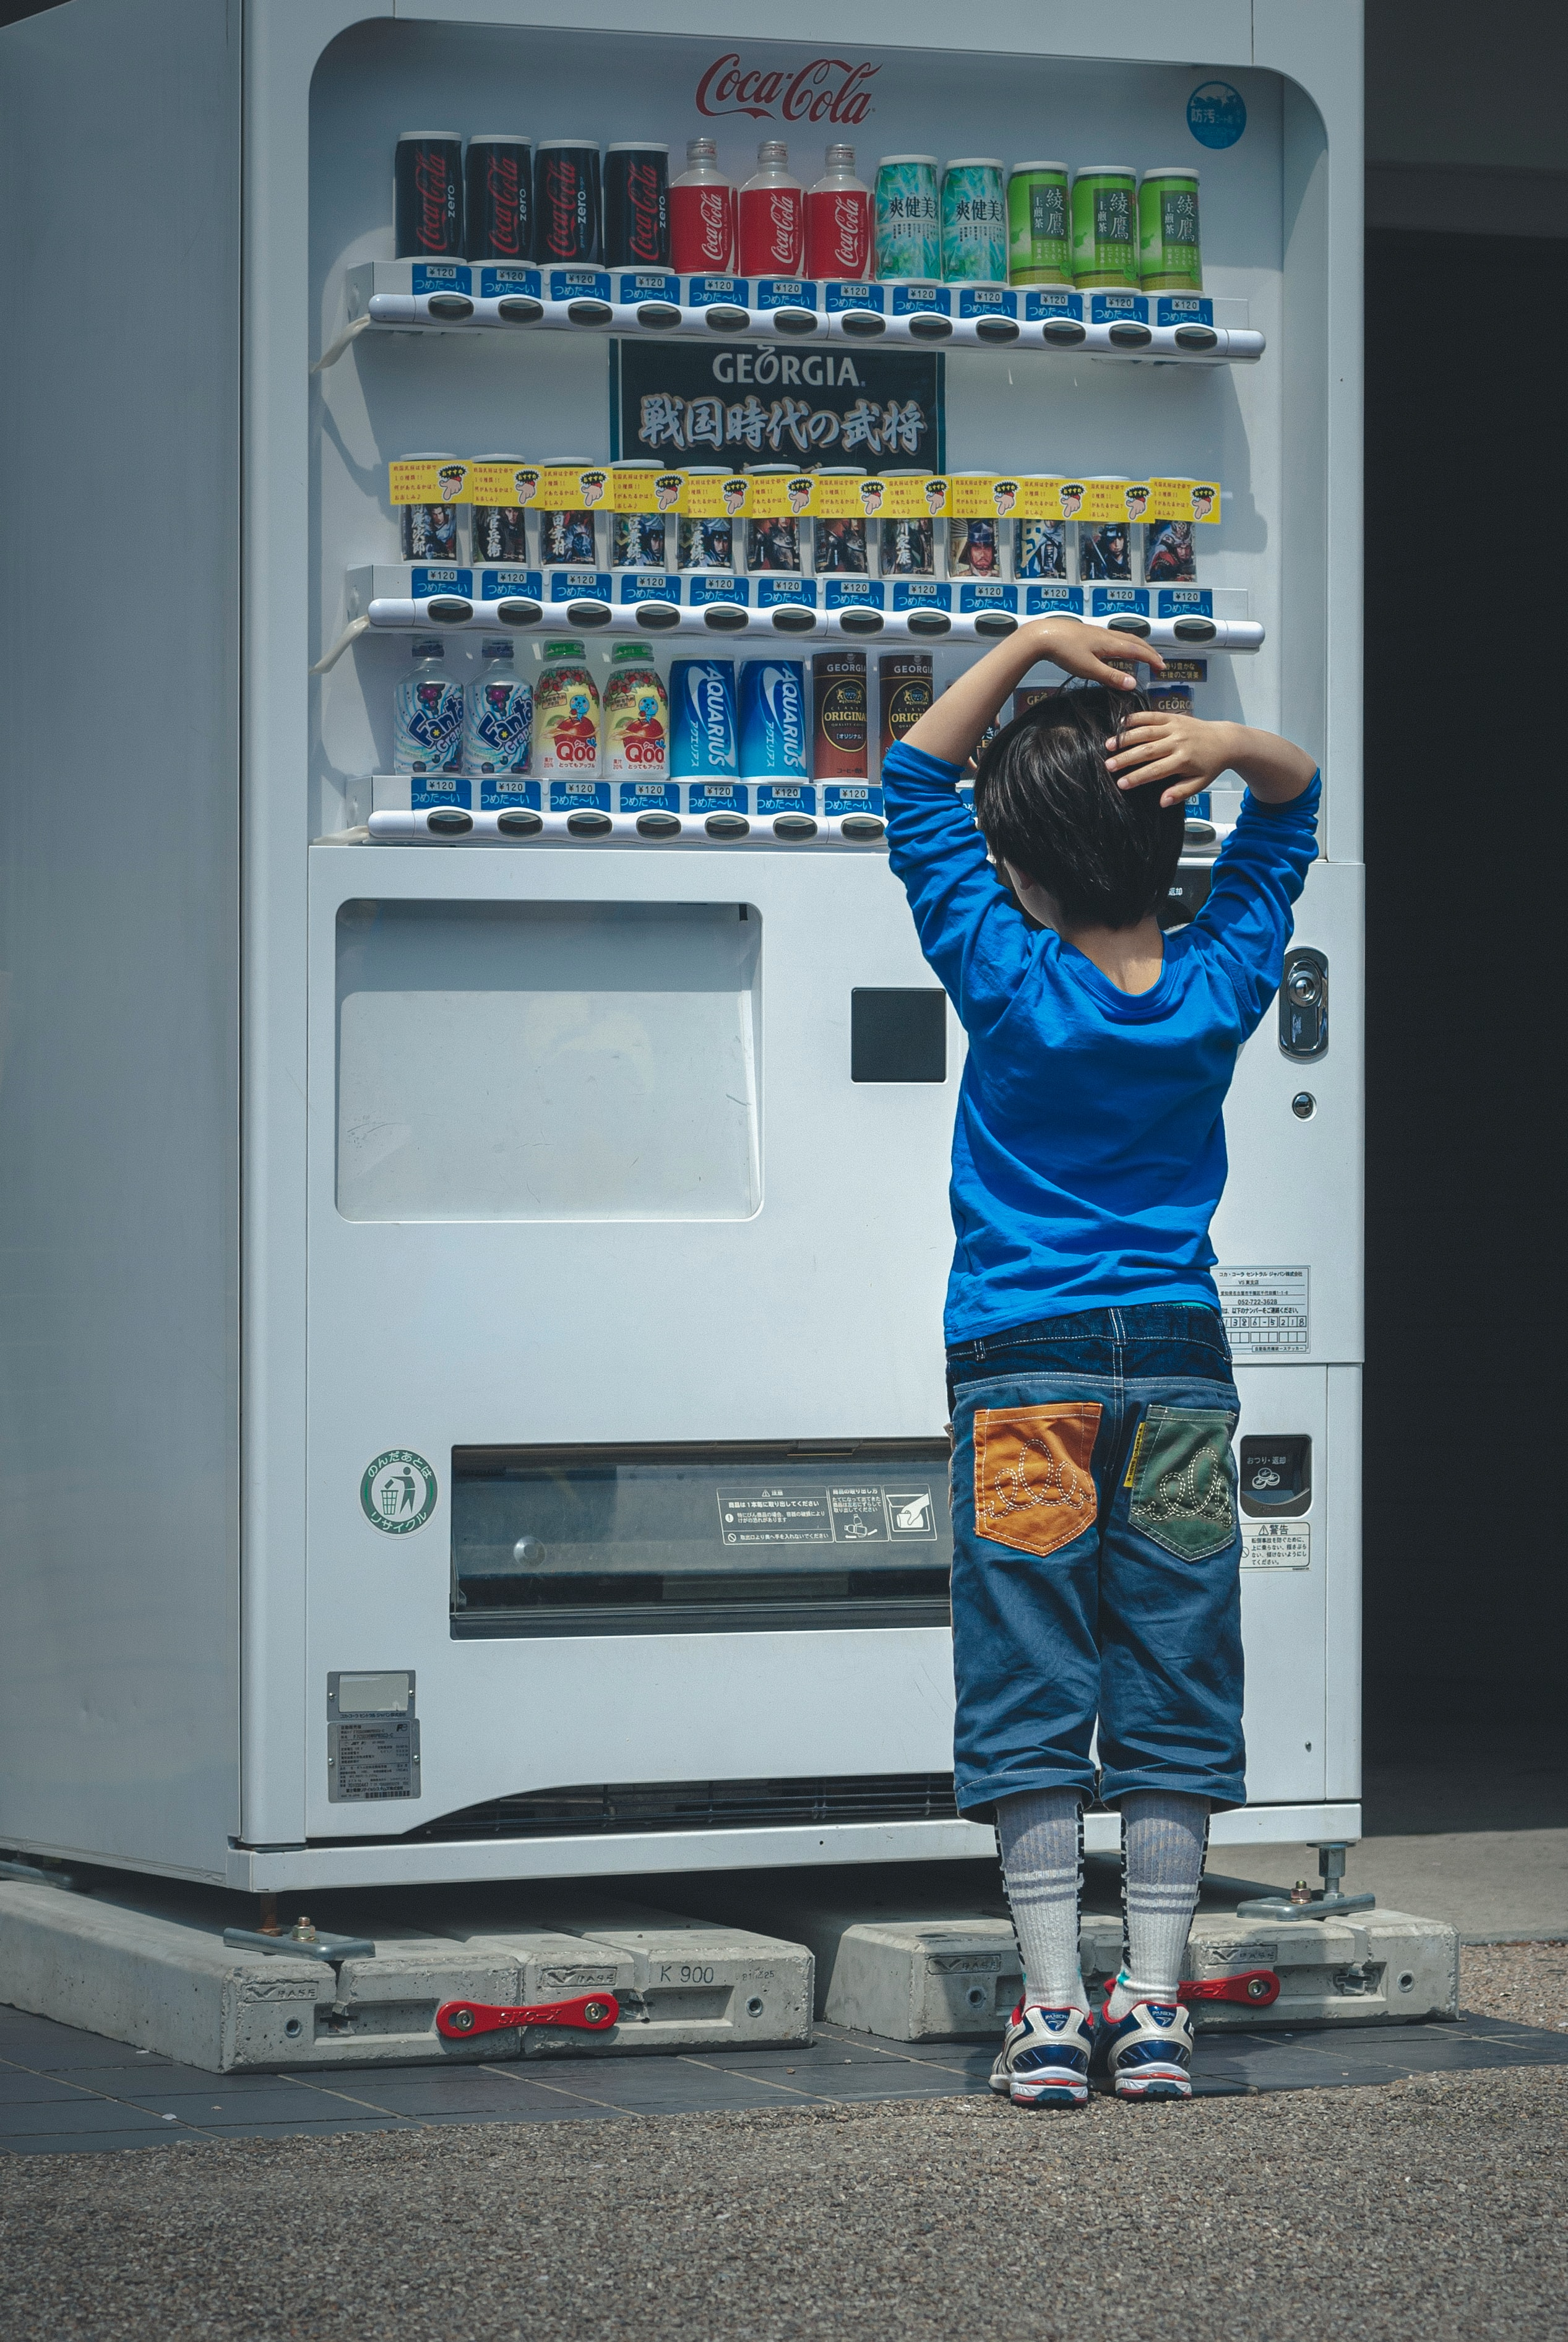
\includegraphics[width=0.85\linewidth]{images/1_i_sistemi/vending_machine.jpg}
%			\caption{}
			\label{fig:systems_vendingmachine}
		\end{figure}
		
	\end{columns}
	
\end{frame}


\subsubsection[Proprio o improprio]{Proprio o improprio}
\begin{frame}
	\frametitle{Proprio o improprio}
	\begin{block}{Un sistema è \textbf{proprio}}
		quando l'uscita dipende solo dallo stato e non dall'ingresso nello stesso istante.
	\end{block}
	
	\begin{block}{Un sistema è \textbf{improprio}}
		quando l'ingresso influenza la formazione del valore d'uscita anche nello stesso istante.
	\end{block}
	
	\begin{columns}			
		\column{0.5\linewidth}
		\begin{figure}[!htbp] 
			\centering
			%\advance\leftskip-0.25cm
			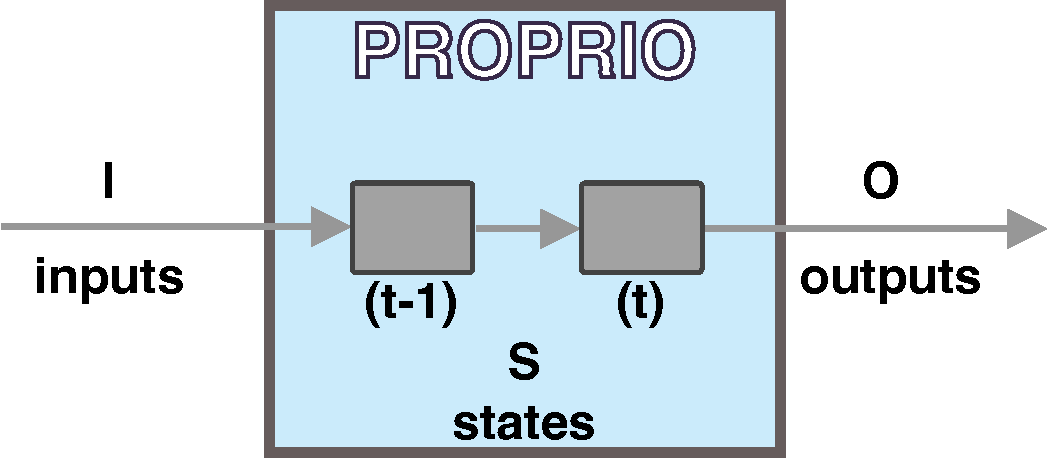
\includegraphics[width=1.0\linewidth]{images/1_i_sistemi/systemProprio.pdf}
					%\caption{}
		\end{figure}
					
		\column{0.5\linewidth}
		\begin{figure}[!htbp] 
			\centering
			%\advance\leftskip-0.25cm
			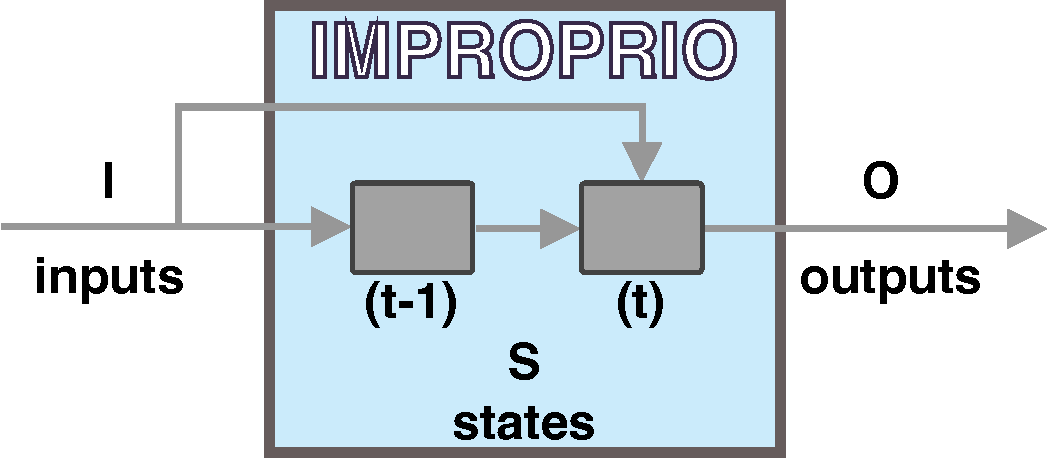
\includegraphics[width=1.0\linewidth]{images/1_i_sistemi/systemImproprio.pdf}
					%\caption{}
		\end{figure}
		
	\end{columns}
	
\end{frame}


\begin{frame}
	\frametitle{Proprio o improprio}
	
	\begin{block}{Esempio di un sistema \textbf{proprio}}
		Un sistema di illuminazione è un sistema proprio in quanto le uscite (luce delle lampadine) sono direttamente dipendenti dallo stato del sistema.	
		
		\begin{figure}[!htbp]
			\centering 
			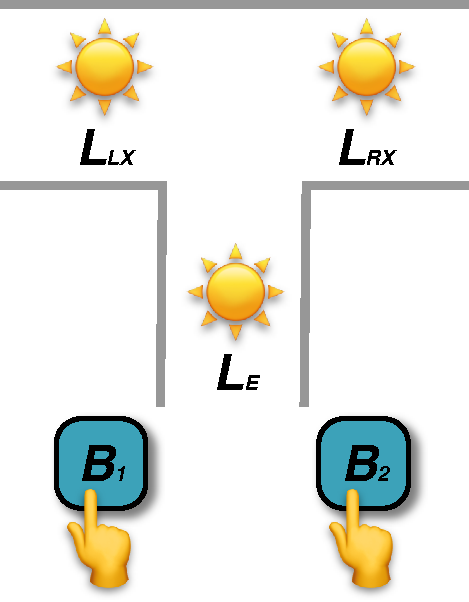
\includegraphics[width=0.3\linewidth]{images/1_i_sistemi/sistemaLight.pdf}
					%\caption{}
		\end{figure}
	\end{block}
	
	
\end{frame}



\subsubsection[I modelli]{I modelli}
\begin{frame}
	\frametitle{La modellazione dei sistemi}
	\begin{block}{I sistemi reali}
		I \textbf{sistemi reali sono complessi da studiare}, e sono spesso costituiti da numerosi elementi che possono essere legati da relazioni non sempre intuitive.
		\textbf{Per studiare un sistema} è necessario utilizzare un \textbf{modello} che ne simuli il comportamento. 
	\end{block}
	
	\begin{block}{Il modello}
		Il \textbf{modello} di un sistema è un insieme di elementi che permettono di riprodurre, valutare o stimare, anche limitatamente ad un certo contesto, le funzioni svolte dal sistema originale, in maniera \textbf{più semplice} senza dover per forza intervenire su di esso.
		Nel modello si focalizza l’attenzione sugli \textbf{elementi essenziali}, \textbf{trascurando i dettagli} che non portano informazioni e ne rendono lo studio eccessivamente complesso.
%		L'idea è quella di sostituire il sistema reale con una sua rappresentazione integrale che metta in evidenza solo gli elementi che si ritengono utili allo scopo dell'analisi.
	\end{block}
	
	
\end{frame}


\subsection[Il computer]{Il computer}
\begin{frame}
	\frametitle{Il sistema computer}
	
	\begin{columns}			
		\column{0.6\linewidth}
		\begin{block}{Il computer}
			I computer è a tutti gli effetti un sistema complesso che potremmo classificare come invariante, deterministico, discreto...\\
			Affinché noi possiamo carpirne gli elementi essenziali è necessario studiare tale sistema attraverso un modello.\\~\\
			In seguito vedremo quali sono alcuni dei modelli più utilizzati per iniziare a studiare il funzionamento del sistema-computer.			
		\end{block}
		
		\column{0.4\linewidth}
		\begin{figure}[!htbp]
			\centering 
			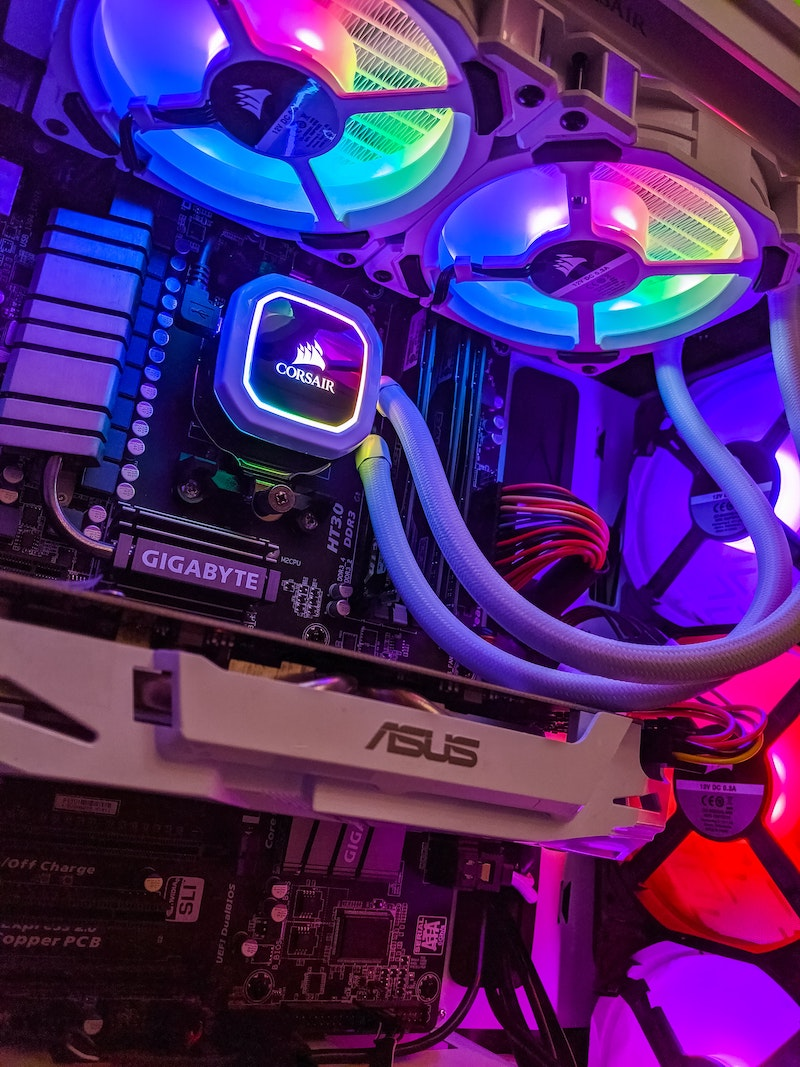
\includegraphics[width=0.95\linewidth]{images/1_i_sistemi/computer.jpeg}
			\label{fig:systems_computer}
		\end{figure}		
	\end{columns}
	
	
\end{frame}

\section[Le architetture]{Le architetture}
\sectionframe{images/covers/cover_architecture.jpeg}{Le Architetture}
% Seattle Public Library Central Library, Seattle, United States: https://unsplash.com/it/foto/if2coegqwZU by Chance Anderson

\subsection[L'architettura di un computer]{L'architettura di un computer}


\begin{frame}
	\frametitle{L'architettura di un computer}
	 
	\begin{block}{}
	
	\end{block}
	\begin{block}{}
	
	\end{block}
\end{frame}


\section[Credits]{Credits}
\sectionframe{images/covers/cover_architecture.jpeg}{Le Architetture}
% 

\newcommand{\photoref}[4]{Fig. \ref{#1}, pag. \pageref{#1}: photo by \href{#3}{#2}, \href{#4}{link}}

\begin{frame}

	\textbf{\nameref{sec:systems}}:
	\begin{itemize}
		\item \photoref{sec:systems}{Jay Mantri}{https://jaymantri.com/}{https://jaymantri.com/post/104375101928/download}
		\item \photoref{fig:systems_vendingmachine}{Egor Myznik}{https://unsplash.com/it/@vonshnauzer}{https://unsplash.com/it/foto/DRs9XsNlAZw}
		\item \photoref{fig:systems_computer}{Andy Holmes}{https://unsplash.com/it/@andyjh07}{https://unsplash.com/it/foto/EOAKUQcsFIU}
	\end{itemize}
	
	
	\textbf{\nameref{sec:architectures}}:
	\begin{itemize}
		\item \photoref{sec:architectures}{Chance Anderson}{https://unsplash.com/it/@chanceanderson}{https://unsplash.com/it/foto/if2coegqwZU}, Seattle Public Library Central Library, Seattle, United States
	\end{itemize}
	
\end{frame}


 


\end{document}
